\subsection{Restriction of a measure to an open set. Definition of a measure by means of local data}

Let X be a locally compact space, Y an open set in X. The subspace Y of X is locally compact, and every continuous function with values in a topological vector space E, defined on Y and with compact support, may be extended by continuity to all of X, by giving it the value 0 on \(\complement \mathrm{Y}\); one can therefore identify in this way the space \(\mathcal{K}(\mathrm{Y};\mathrm{E})\) with the linear subspace of \(\mathcal{K}(\mathrm{X};\mathrm{E})\) formed by the continuous functions with compact support contained in Y. If \(\mu\) is a measure on X, it is clear that the restriction of \(\mu\) to \(\mathcal{K}(\mathrm{Y};\mathbf{C})\) is a measure on Y, which is called the restriction of \(\mu\) to the open subspace Y, or the measure induced on Y by \(\mu\) , and is denoted \(\mu|\mathrm{Y}\) . The restrictions to Y of \(|\mu|\) , \(\mathcal{R}\mu\) and \(\mathcal{I}\mu\) are, respectively, \(|\mu|\mathrm{Y}|\) , \(\mathcal{R}(\mu|\mathrm{Y})\) and \(\mathcal{I}(\mu|\mathrm{Y})\) , by virtue of §1, Nos. 5 and 6. If \(\mu\) is real then the restrictions of \(\mu^{+}\) and \(\mu^{-}\) to Y are, respectively, \((\mu|\mathrm{Y})^{+}\) and \((\mu|\mathrm{Y})^{-}\) , by virtue of formula (8) of §1, No.~5.

One sees immediately that if Y and Z are two open sets in X such that \(Y \supset Z\) , and if \(\mu|Y\) and \(\mu|Z\) are the restrictions of \(\mu\) to Y and Z, then \(\mu|Z\) is also the restriction of \(\mu|Y\) to the open subspace Z of the locally compact space Y.

In Ch. IV, §5, No.~7 we shall generalize this definition to the case that Y is a locally compact subspace of X.

\pandocbounded{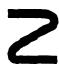
\includegraphics[keepaspectratio]{images/part001_8e0e9629.jpg}}

Note that a measure on Y is not necessarily the restriction of some measure on X (cf.~Ch. V, §7, No.~2, Prop. 3).

For example, let Y be the open interval {]}0,1{[} of X = R; the mapping

\[
f \mapsto \int_ {0} ^ {1} \frac {f (x)}{x} d x
\]

is a measure on Y, because every function in \(\mathcal{K}(\mathrm{Y};\mathbf{C})\) is zero on a neighborhood of 0 in \(\mathbf{R}\) . However, this measure cannot be extended to a measure on \(\mathbf{R}\) because, in the contrary case, its restriction to the set of functions \(f\in \mathcal{K}(\mathrm{Y};\mathbf{C})\) such that \(\| f\| \leqslant 1\) would be bounded; but this is false.

However, we have the following proposition:

PROPOSITION 1. --- Let \((\mathrm{Y}_{\alpha})_{\alpha\in\mathrm{A}}\) be an open covering of X and suppose given, on each subspace \(Y_{\alpha}\) , a measure \(\mu_{\alpha}\) , in such a way that for every pair \((\alpha,\beta)\) , the restrictions of \(\mu_{\alpha}\) and \(\mu_{\beta}\) to \(Y_{\alpha}\cap Y_{\beta}\) are identical. Under these conditions, there exists one and only one measure \(\mu\) on X whose restriction to \(Y_{\alpha}\) is equal to \(\mu_{\alpha}\) for every index \(\alpha\) .

Let us first show that every function \(f \in \mathcal{K}(\mathrm{X};\mathbf{C})\) may be written in the form of a finite sum \(f = \sum_{i} f_{i}\) where, for each of the functions \(f_{i} \in \mathcal{K}(\mathrm{X};\mathbf{C})\) , there exists an index \(\alpha_{i}\) such that \(\operatorname{Supp}(f_{i}) \subset \mathrm{Y}_{\alpha_{i}}\) . If \(\mathrm{K} = \operatorname{Supp}(f)\) , there exists a finite number of indices \(\alpha_{i} (1 \leqslant i \leqslant n)\) such that the \(\mathrm{Y}_{\alpha_{i}}\) form a covering of \(\mathrm{K}\) ; let \(h_{i} (1 \leqslant i \leqslant n)\) be continuous mappings of \(\mathrm{X}\) into {[}0,1{]} such that the support of \(h_{i}\) is compact and is contained in \(\mathrm{Y}_{\alpha_{i}}\) for \(1 \leqslant i \leqslant n\) , and such that \(\sum_{i=1}^{n} h_{i}(x) = 1\) on \(\mathrm{K} (\S 1, \text{No. 2, Lemma 1})\) ; the functions \(f_{i} = f h_{i}\) meet the requirements. This shows in the first place that if there exists a measure \(\mu\) meeting the requirements then it is unique, because for every finite sum \(f = \sum_{i=1}^{n} f_{i}\) , where \(f_{i} \in \mathcal{K}(\mathrm{Y}_{\alpha_{i}}; \mathbf{C})\) , necessarily \(\mu(f) = \sum_{i=1}^{n} \mu_{\alpha_{i}}(f_{i})\) . Moreover, we will have shown the existence of a linear form \(\mu\) on \(\mathcal{K}(\mathrm{X};\mathbf{C})\) whose restriction to each subspace \(\mathcal{K}(\mathrm{Y}_{\alpha};\mathbf{C})\) is \(\mu_{\alpha}\) , provided we demonstrate the following property: if \((g_{i})_{1 \leqslant i \leqslant m}\) and \((h_{j})_{1 \leqslant j \leqslant n}\) are two finite sequences of functions in \(\mathcal{K}(\mathrm{X};\mathbf{C})\) such that \(g_{i} \in \mathcal{K}(\mathrm{Y}_{\alpha_{i}}; \mathbf{C})\) for \(1 \leqslant i \leqslant m\) , \(h_{j} \in \mathcal{K}(\mathrm{Y}_{\beta_{j}}; \mathbf{C})\) for \(1 \leqslant j \leqslant n\) and

\[
\sum_ {i = 1} ^ {m} g _ {i} (x) = \sum_ {j = 1} ^ {n} h _ {j} (x) = 1
\]

on K, then

\[
\sum_ {i = 1} ^ {m} \mu_ {\alpha_ {i}} (f g _ {i}) = \sum_ {j = 1} ^ {n} \mu_ {\beta_ {j}} (f h _ {j}).
\]

Now,

\[
f g _ {i} = \sum_ {j = 1} ^ {n} f g _ {i} h _ {j},
\]

whence

\[
\sum_ {i = 1} ^ {m} \mu_ {\alpha_ {i}} (f g _ {i}) = \sum_ {i = 1} ^ {m} \sum_ {j = 1} ^ {n} \mu_ {\alpha_ {i}} (f g _ {i} h _ {j}).
\]

Similarly,

\[
\sum_ {j = 1} ^ {n} \mu_ {\beta_ {j}} (f h _ {j}) = \sum_ {j = 1} ^ {n} \sum_ {i = 1} ^ {m} \mu_ {\beta_ {j}} (f g _ {i} h _ {j}).
\]

But since the support of \(fg_{i}h_{j}\) is contained in \(\mathbf{Y}_{\alpha_i}\cap \mathbf{Y}_{\beta_j}\) , we have \(\mu_{\alpha_i}(fg_i h_j) = \mu_{\beta_j}(fg_i h_j)\) , which establishes our assertion.

It remains to see that \(\mu\) is a measure on X; now, every point of X admits a compact neighborhood contained in one of the \(Y_{\alpha}\) ; the conclusion therefore follows at once from the definition of \(\mu\) and from Prop. 6 of §1, No.~3.

COROLLARY (Principle of localization). --- Let \(\mu\) and \(\nu\) be two measures on X, and let \((\mathrm{Y}_{\alpha})\) be a family of open sets of X such that, for every \(\alpha\) , the restrictions to \(Y_{\alpha}\) of \(\mu\) and \(\nu\) are equal; then the restrictions of \(\mu\) and \(\nu\) to \(Y = \bigcup_{\alpha} Y_{\alpha}\) are equal.

